\setcounter{chapter}{1}
\chapter{PREVIOUS WORK} \label{previousWork}

\section{Section Example}

\begin{table}[H]
	\begin{center} {\footnotesize
			\begin{tabular}{ccc}
		\hline 
		\textbf{Index} & \textbf{Columns }\\
		\hline
		\rowcolor{blue!20}0 & Blue  \\
		\rowcolor{black!0}1 & White  \\
		\rowcolor{blue!20}0 & Blue  \\
		\rowcolor{black!0}1 & White  \\
		

\end{tabular}}
\end{center}
\caption{\footnotesize Fancy Table}
\label{fancyTable}
\end{table}

Example:

\textbf{\centerline{
$\bigl[ \begin{matrix}
N^{\circ} Examples,  & N^{\circ} Examples, & Example\\
\end{matrix} \bigr]$}}

\section{Section example }
Paragraph
\begin{itemize}
	\item List 1 with image 

\begin{figure}[H]
	\centering
	{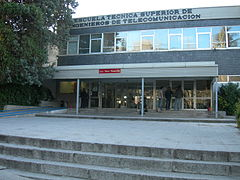
\includegraphics[width=.95\textwidth,height=0.25\textheight]{UPM-ETSIT--Sanz_Mancebo} }
	\caption{Image within a list}%
	\label{fig:image in a list}
\end{figure}


\end{itemize}

\section{Icon Section \protect\icon{android}}\label{sec:iconsection}

\subsection{Subsection example}
Paragraph...